\documentclass{beamer}

%Russian-specific packages
%--------------------------------------
\usepackage[T2A]{fontenc}
\usepackage[utf8]{inputenc}
\usepackage[english,main=russian]{babel}
%--------------------------------------

\usepackage{graphicx}
\usepackage{amssymb,amsmath}
\usepackage{pgfplots, pgfplotstable}
\pgfplotsset{compat=newest}
\makeatletter
\pgfplotsset{
    /pgfplots/flexible xticklabels from table/.code n args={3}{%
        \pgfplotstableread[#3]{#1}\coordinate@table
        \pgfplotstablegetcolumn{#2}\of{\coordinate@table}\to\pgfplots@xticklabels
        \let\pgfplots@xticklabel=\pgfplots@user@ticklabel@list@x
    }
}
\makeatother
\definecolor{basicno}{rgb}{0.624,0.0,0.0}
\definecolor{basicsome}{rgb}{0.424,0.0,0.0}
\definecolor{random}{rgb}{0.0,0.100,0.424}
\definecolor{gena}{rgb}{0.0,0.100,0.624}
\definecolor{heuno}{rgb}{0.2,0.524,0.2}
\definecolor{heusome}{rgb}{0.2,0.424,0.2}
\definecolor{heumore}{rgb}{0.1,0.324,0.1}

\graphicspath{{logo/}{pics/}}
\beamertemplatenavigationsymbolsempty{}
\setbeamertemplate{footline}[frame number]
\setbeamerfont{footline}{size={\fontsize{10}{12}}}

\title{Оптимизация функции, задаваемой регрессионным лесом}
\author{Влад Ягламунов}
\date{}

\begin{document}

\begin{frame}
\maketitle
{\small 
    \textbf{Формальный научный руководитель:}\par Фильченков Андрей Александрович\par
    \textbf{Фактический научный руководитель:}\par Шаламов Вячеслав Владимирович
}
\end{frame}

\begin{frame} \frametitle{Задача}
    \begin{itemize}
        \item \textbf{Дано:} Обученный регрессионный лес
        \item \textbf{Найти:} Области, где лес возвращает минимальное и максимальное значение
    \end{itemize}
\end{frame}

\begin{frame} \frametitle{Применение}
    Random Forest:
    \begin{itemize}
        \item Суррогатные функции для оптимизации
        \item Хорошо обновляется при добавлении информации \pause{}
        \item Последовательная оптимизация основанная на модели Sequential Model-Based Optimization (SMBO)
        \item Sequential Model-based Algorithm configuration (SMAC)
    \end{itemize}
    \vfill
    \pause{}
    Сейчас используется перебор случайного набора точек.
    \vfill
\end{frame}

\begin{frame} \frametitle{Random Forest}
    \begin{columns}
        \column{.6\textwidth}
            \begin{itemize}
                \item Ансамбль деревьев принятия решения
                \item Каждое дерево обучено на случном подмножестве
                \item Результат: среднее всех деревьев 
                \item Пространство разбивается на прямоугольники по границам разбиения вершин
            \end{itemize}
        \column{.4\textwidth}
        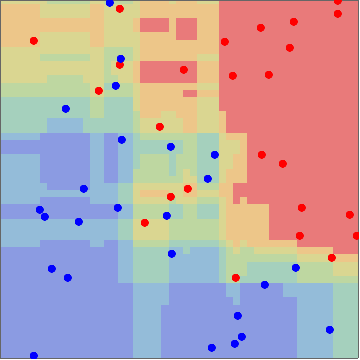
\includegraphics[width=\textwidth]{random_forest.png}
    \end{columns}
\end{frame}

\begin{frame} \frametitle{Эвристический алгоритм}
    \begin{columns}
        \column{.5\textwidth}
            \begin{itemize}
                \item Перебор по всем поддеревьям
                \item Для вершины храним минимум и максимум в поддереве
                \item Поддерживаем, что все поддеревья пересекаются
            \end{itemize}
        \column{.5\textwidth}
            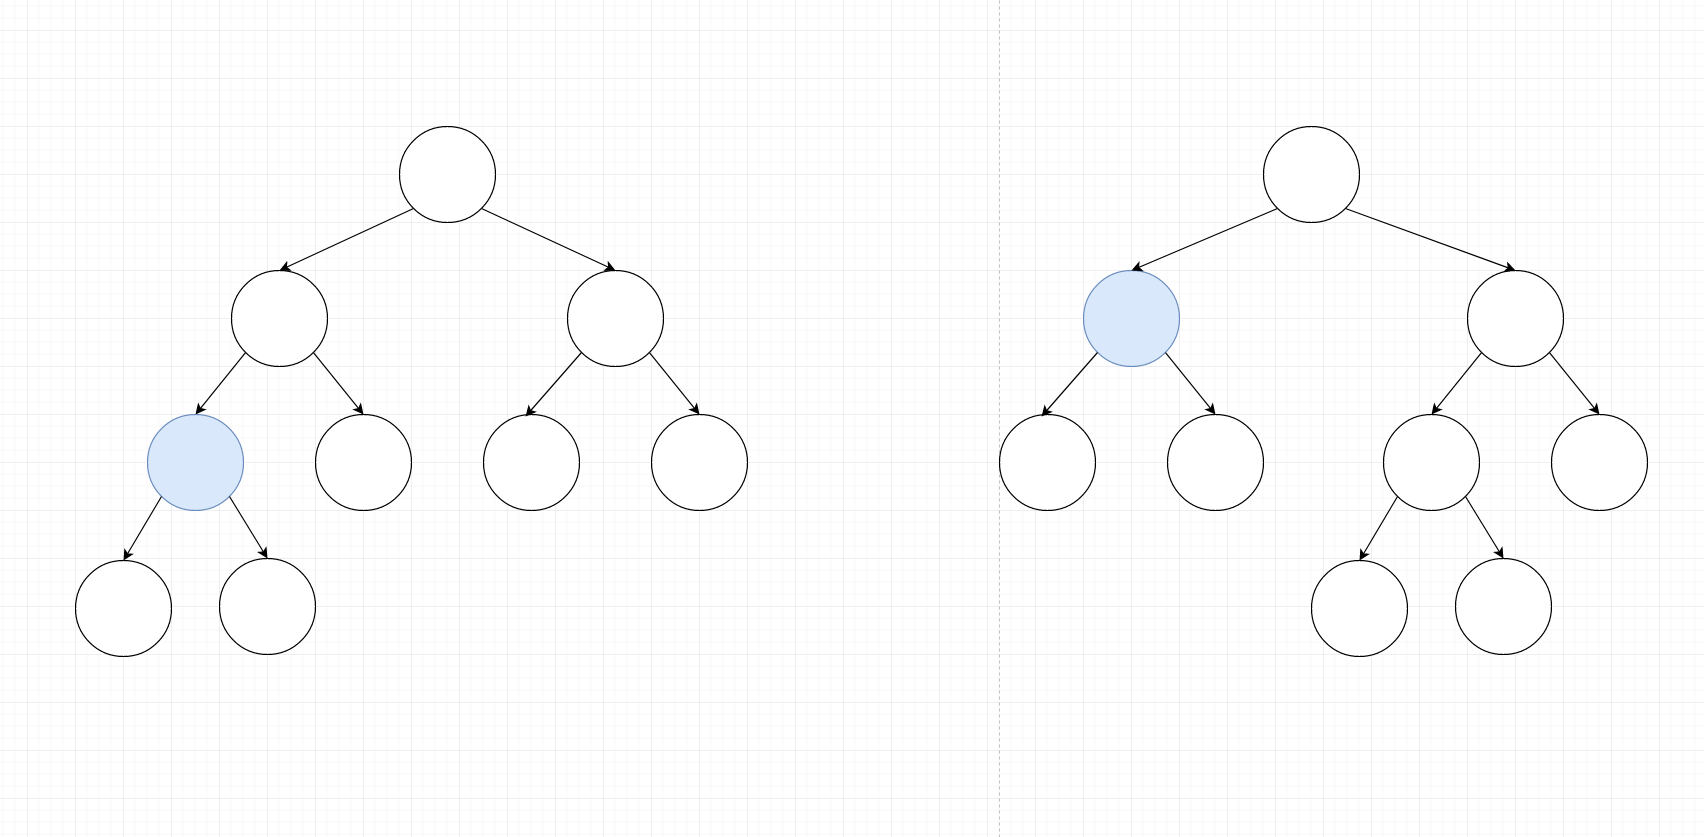
\includegraphics[width=\textwidth]{tree.png}
    \end{columns}
\end{frame}

\begin{frame} \frametitle{Эвристический алгоритм}

    \begin{columns}
        \column{.75\textwidth}
            На каждом шаге рассматриваем n-мерный прямоугольник области

            Шаг: разбиение по границе вершины
        \column{.25\textwidth}
            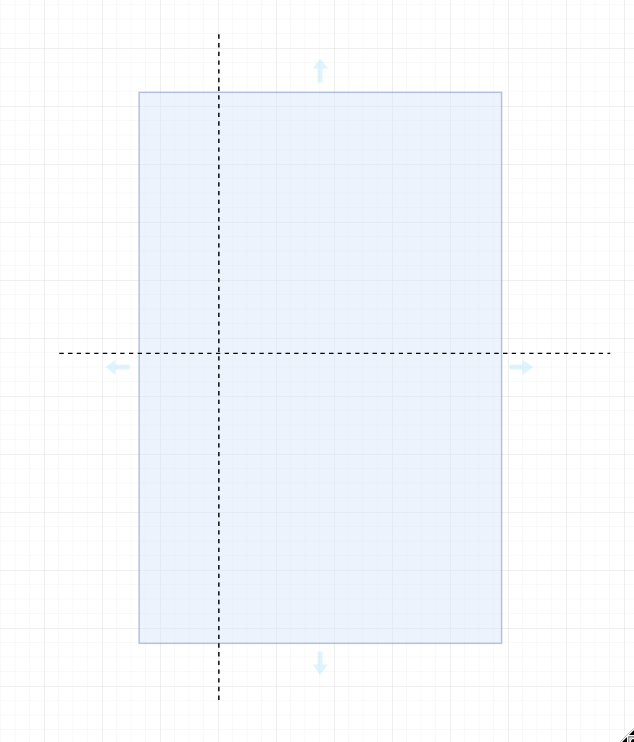
\includegraphics[width=\textwidth]{split.png}
    \end{columns}
    \vfill
    \pause{}
    Эвристика:
    \[
        i = \arg \max_{v \in trees}(|value[v.left] - value[v.right]|)
    \]
\end{frame}

\begin{frame} \frametitle{Эвристический алгоритм (Оптимизация 1)}
    Необязательно искать точное решение.

    \vspace{50px}
    Не будем перебирать поддерево, если в лучшем случае это не улучшит ответ хотя бы на $\alpha$

    \[
        value[v] < \alpha current
    \]

    Гарантирует точность $>\alpha$
\end{frame}

\begin{frame} \frametitle{Эвристический алгоритм (Оптимизация 2)}
    Максимум в поддереве может не пересекаться с текущей областью

    \begin{columns}
        \column{.5\textwidth}
            \begin{itemize}
                \item Отсортированный список всех его листьев
                \item На каждом шаге в таком списке мы движемся только вперёд
            \end{itemize}
        \column{.5\textwidth}
            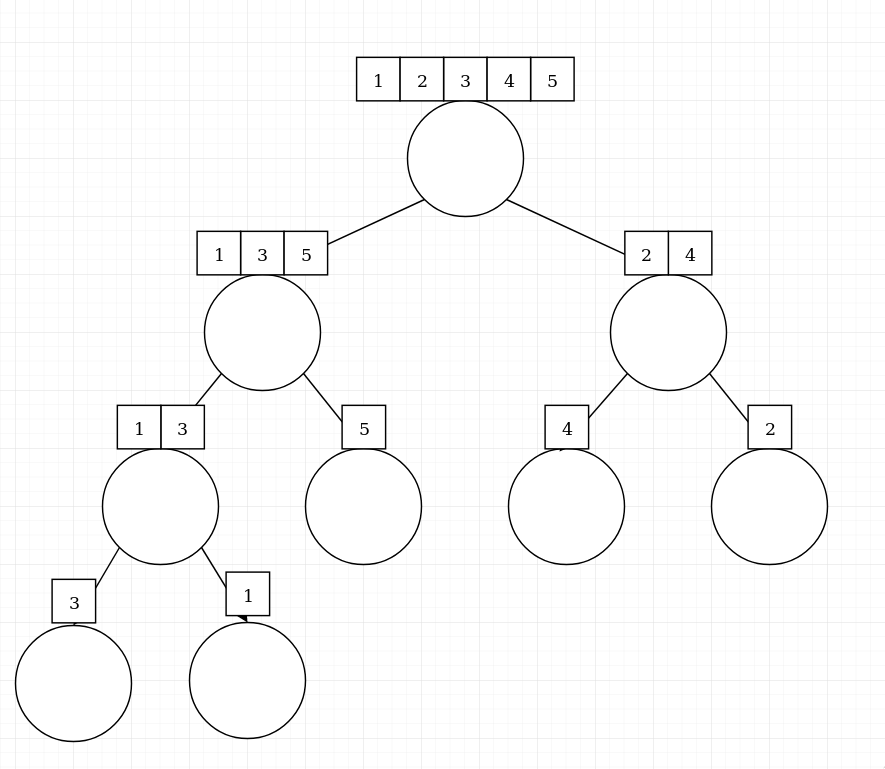
\includegraphics[width=1.1\textwidth]{merge.png}
    \end{columns}
\end{frame}

\begin{frame} \frametitle{Алгоритм имитации отжига}
    \begin{center}
    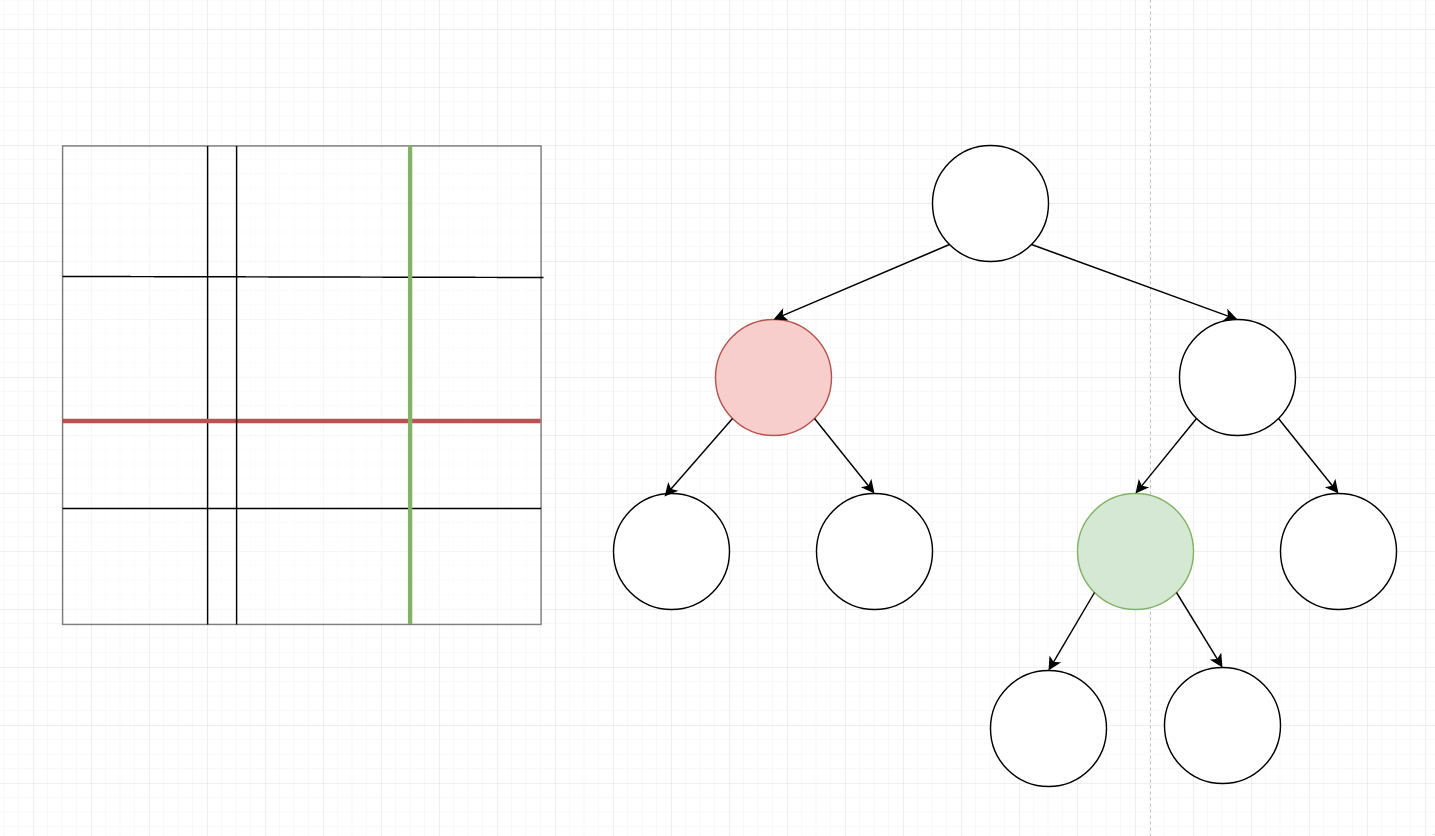
\includegraphics[width=0.8\textwidth]{gena.png}
    \end{center}
    \begin{itemize}
        \item Разбиваем пространство по всем границам
        \item Случайные мутации по переходе в соседнюю клетку
        \item Достаточно пересчитать только одно дерево
    \end{itemize}
\end{frame}

\begin{frame} \frametitle{Алгоритм имитации отжига}
\begin{columns}
    \column{.5\textwidth}
    Если значение ухудшилось, то переходим с вероятностью уменьшающейся от температуры (номера итерации)
    \[
    p=\alpha + (1 - \alpha) \frac{i}{N}
    \]
    N --- количество итераций\\
    i --- номер итераций
    \column{.5\textwidth}
    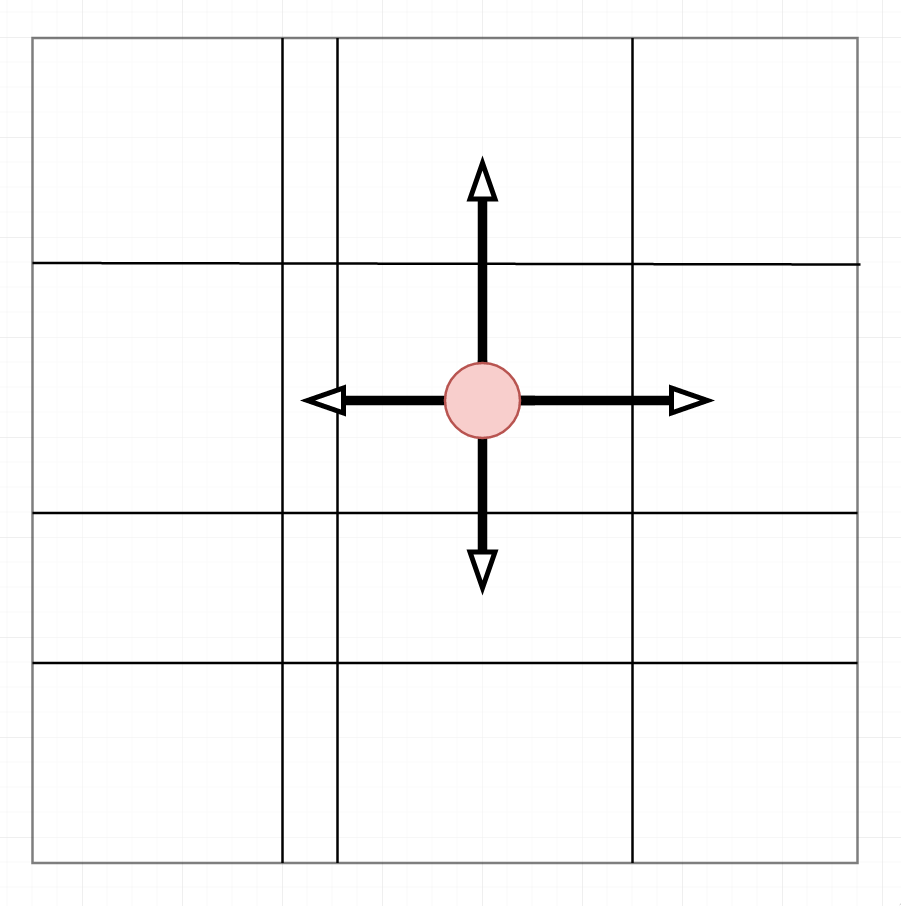
\includegraphics[width=\textwidth]{gena_move.png}
\end{columns}
\end{frame}

\begin{frame} \frametitle{Сравниваемые алгоритмы}
    \begin{itemize}
        \item Перебор
        \item Перебор с погрешностью $<5\%$
        \item Случайный
        \item Отжиг
        \item Эвристика
        \item Эвристика с погрешностью $<5\%$
        \item Эвристика с погрешностью $<15\%$
    \end{itemize}
\end{frame}

\begin{frame} \frametitle{Использованные данные}
    Использованные различные общедоступные датасеты с OpenML

    \vfill
    \begin{center}
        \begin{tabular}{|l|l|l|}

        \hline

        название        & элементы  & признаки \\

        \hline

        diabetes        & 442    & 9     \\
        boston          & 506    & 12    \\
        autoPrice       & 159    & 16    \\
        wisconsin       & 194    & 33    \\
        strikes         & 625    & 7     \\
        kin8nm          & 8192   & 9     \\
        house\_8L       & 22784  & 9     \\
        house\_16H      & 22784  & 9     \\
        mtp2            & 274    & 1143  \\

        \hline

    \end{tabular}

    \vfill
    На каждом наборе параметров проводилось 10 тестов.
    \end{center}
\end{frame}

\begin{frame} \frametitle{Тестирование (Время работы | Простой случай)}
    \pgfplotstableread[col sep=comma]{../data/easy/basic-00.csv}\basicno
    \pgfplotstableread[col sep=comma]{../data/easy/basic-05.csv}\basicsome
    \pgfplotstableread[col sep=comma]{../data/easy/heuristic-00.csv}\heuno
    \pgfplotstableread[col sep=comma]{../data/easy/heuristic-05.csv}\heusome
    \pgfplotstableread[col sep=comma]{../data/easy/heuristic-15.csv}\heumore
    \pgfplotstableread[col sep=comma]{../data/easy/random.csv}\random
    \pgfplotstableread[col sep=comma]{../data/easy/gena.csv}\gena

    \begin{center}
    \begin{tikzpicture}
    \begin{axis}[
        enlarge x limits=0.2,
        ybar=0pt, 
        width=1\textwidth,
        height=0.8\textwidth,
        bar width=8pt,
        ymin=0,
        xlabel=Датасет,
        ylabel=Время работы,
        flexible xticklabels from table={../data/easy/heuristic-15.csv}{algo}{col sep=comma},
        xticklabel style={text height=1.5ex, font=\tiny}, % To make sure the text labels are nicely aligned
        xtick=data,
    ]
    \addplot 
        [color=basicno, fill=basicno, fill opacity=0.33]
        plot [error bars/.cd, error bar style={line width=1pt}, y dir = both, y explicit]
        table[x expr=\coordindex, y=mean_time, y error=std_time]{\basicno};
    \addplot 
        [color=basicsome, fill=basicsome, fill opacity=0.33]
        plot [error bars/.cd, error bar style={line width=1pt}, y dir = both, y explicit]
        table[x expr=\coordindex, y=mean_time, y error=std_time]{\basicsome};
    \addplot 
        [color=random, fill=random, fill opacity=0.33]
        plot [error bars/.cd, error bar style={line width=1pt}, y dir = both, y explicit]
        table[x expr=\coordindex, y=mean_time, y error=std_time]{\random};
    \addplot 
        [color=gena, fill=gena, fill opacity=0.33]
        plot [error bars/.cd, error bar style={line width=1pt}, y dir = both, y explicit]
        table[x expr=\coordindex, y=mean_time, y error=std_time]{\gena};
    \addplot 
        [color=heuno, fill=heuno, fill opacity=0.33]
        plot [error bars/.cd, error bar style={line width=1pt}, y dir = both, y explicit]
        table[x expr=\coordindex, y=mean_time, y error=std_time]{\heuno};
    \addplot 
        [color=heusome, fill=heusome, fill opacity=0.33]
        plot [error bars/.cd, error bar style={line width=1pt}, y dir = both, y explicit]
        table[x expr=\coordindex, y=mean_time, y error=std_time]{\heusome};
    \addplot 
        [color=heumore, fill=heumore, fill opacity=0.33]
        plot [error bars/.cd, error bar style={line width=1pt}, y dir = both, y explicit]
        table[x expr=\coordindex, y=mean_time, y error=std_time]{\heumore};

    \legend{%
        Перебор, 
        Перебор с $<5\%$, 
        Случайный, 
        Отжиг, 
        Эвристика, 
        Эвристика с $<5\%$, 
        Эвристика с $<15\%$ 
    }

    \end{axis}
    \end{tikzpicture}
    \end{center}
\end{frame}

\begin{frame} \frametitle{Тестирование (Время работы | Много деревьев)}
    \pgfplotstableread[col sep=comma]{../data/trees/basic-00.csv}\basicno
    \pgfplotstableread[col sep=comma]{../data/trees/basic-05.csv}\basicsome
    \pgfplotstableread[col sep=comma]{../data/trees/heuristic-00.csv}\heuno
    \pgfplotstableread[col sep=comma]{../data/trees/heuristic-05.csv}\heusome
    \pgfplotstableread[col sep=comma]{../data/trees/heuristic-15.csv}\heumore
    \pgfplotstableread[col sep=comma]{../data/trees/random.csv}\random
    \pgfplotstableread[col sep=comma]{../data/trees/gena.csv}\gena

    \begin{center}
    \begin{tikzpicture}
    \begin{axis}[
        enlarge x limits=0.2,
        ybar=0pt, 
        width=1\textwidth,
        height=0.8\textwidth,
        bar width=8pt,
        ymin=0,
        xlabel=Датасет,
        ylabel=Время работы,
        flexible xticklabels from table={../data/trees/heuristic-15.csv}{algo}{col sep=comma},
        xticklabel style={text height=1.5ex, font=\tiny}, % To make sure the text labels are nicely aligned
        xtick=data,
    ]
    \addplot 
        [color=basicno, fill=basicno, fill opacity=0.33]
        plot [error bars/.cd, error bar style={line width=1pt}, y dir = both, y explicit]
        table[x expr=\coordindex, y=mean_time, y error=std_time]{\basicno};
    \addplot 
        [color=basicsome, fill=basicsome, fill opacity=0.33]
        plot [error bars/.cd, error bar style={line width=1pt}, y dir = both, y explicit]
        table[x expr=\coordindex, y=mean_time, y error=std_time]{\basicsome};
    \addplot 
        [color=random, fill=random, fill opacity=0.33]
        plot [error bars/.cd, error bar style={line width=1pt}, y dir = both, y explicit]
        table[x expr=\coordindex, y=mean_time, y error=std_time]{\random};
    \addplot 
        [color=gena, fill=gena, fill opacity=0.33]
        plot [error bars/.cd, error bar style={line width=1pt}, y dir = both, y explicit]
        table[x expr=\coordindex, y=mean_time, y error=std_time]{\gena};
    \addplot 
        [color=heuno, fill=heuno, fill opacity=0.33]
        plot [error bars/.cd, error bar style={line width=1pt}, y dir = both, y explicit]
        table[x expr=\coordindex, y=mean_time, y error=std_time]{\heuno};
    \addplot 
        [color=heusome, fill=heusome, fill opacity=0.33]
        plot [error bars/.cd, error bar style={line width=1pt}, y dir = both, y explicit]
        table[x expr=\coordindex, y=mean_time, y error=std_time]{\heusome};
    \addplot 
        [color=heumore, fill=heumore, fill opacity=0.33]
        plot [error bars/.cd, error bar style={line width=1pt}, y dir = both, y explicit]
        table[x expr=\coordindex, y=mean_time, y error=std_time]{\heumore};

    \legend{%
        Перебор, 
        Перебор с $<5\%$, 
        Случайный, 
        Отжиг, 
        Эвристика, 
        Эвристика с $<5\%$, 
        Эвристика с $<15\%$ 
    }

    \end{axis}
    \end{tikzpicture}
    \end{center}
\end{frame}

\begin{frame} \frametitle{Тестирование (Время работы | Большой датасет)}
    \pgfplotstableread[col sep=comma]{../data/big/basic-00.csv}\basicno
    \pgfplotstableread[col sep=comma]{../data/big/basic-05.csv}\basicsome
    \pgfplotstableread[col sep=comma]{../data/big/heuristic-00.csv}\heuno
    \pgfplotstableread[col sep=comma]{../data/big/heuristic-05.csv}\heusome
    \pgfplotstableread[col sep=comma]{../data/big/heuristic-15.csv}\heumore
    \pgfplotstableread[col sep=comma]{../data/big/random.csv}\random
    \pgfplotstableread[col sep=comma]{../data/big/gena.csv}\gena

    \begin{center}
    \begin{tikzpicture}
    \begin{axis}[
        enlarge x limits=0.2,
        ybar=0pt, 
        width=1\textwidth,
        height=0.8\textwidth,
        bar width=8pt,
        ymin=0,
        xlabel=Датасет,
        ylabel=Время работы,
        flexible xticklabels from table={../data/big/heuristic-15.csv}{algo}{col sep=comma},
        xticklabel style={text height=1.5ex, font=\tiny}, % To make sure the text labels are nicely aligned
        xtick=data,
        legend style={at={(0.02,0.98)},anchor=north west},
    ]
    \addplot 
        [color=basicno, fill=basicno, fill opacity=0.33]
        plot [error bars/.cd, error bar style={line width=1pt}, y dir = both, y explicit]
        table[x expr=\coordindex, y=mean_time, y error=std_time]{\basicno};
    \addplot 
        [color=basicsome, fill=basicsome, fill opacity=0.33]
        plot [error bars/.cd, error bar style={line width=1pt}, y dir = both, y explicit]
        table[x expr=\coordindex, y=mean_time, y error=std_time]{\basicsome};
    \addplot 
        [color=random, fill=random, fill opacity=0.33]
        plot [error bars/.cd, error bar style={line width=1pt}, y dir = both, y explicit]
        table[x expr=\coordindex, y=mean_time, y error=std_time]{\random};
    \addplot 
        [color=gena, fill=gena, fill opacity=0.33]
        plot [error bars/.cd, error bar style={line width=1pt}, y dir = both, y explicit]
        table[x expr=\coordindex, y=mean_time, y error=std_time]{\gena};
    \addplot 
        [color=heuno, fill=heuno, fill opacity=0.33]
        plot [error bars/.cd, error bar style={line width=1pt}, y dir = both, y explicit]
        table[x expr=\coordindex, y=mean_time, y error=std_time]{\heuno};
    \addplot 
        [color=heusome, fill=heusome, fill opacity=0.33]
        plot [error bars/.cd, error bar style={line width=1pt}, y dir = both, y explicit]
        table[x expr=\coordindex, y=mean_time, y error=std_time]{\heusome};
    \addplot 
        [color=heumore, fill=heumore, fill opacity=0.33]
        plot [error bars/.cd, error bar style={line width=1pt}, y dir = both, y explicit]
        table[x expr=\coordindex, y=mean_time, y error=std_time]{\heumore};

    \legend{%
        Перебор, 
        Перебор с $<5\%$, 
        Случайный, 
        Отжиг, 
        Эвристика, 
        Эвристика с $<5\%$, 
        Эвристика с $<15\%$ 
    }

    \end{axis}
    \end{tikzpicture}
    \end{center}
\end{frame}

\begin{frame} \frametitle{Тестирование (Ошибка | Простой случай)}
    \pgfplotstableread[col sep=comma]{../data/easy/basic-05.csv}\basicsome
    \pgfplotstableread[col sep=comma]{../data/easy/heuristic-05.csv}\heusome
    \pgfplotstableread[col sep=comma]{../data/easy/heuristic-15.csv}\heumore
    \pgfplotstableread[col sep=comma]{../data/easy/random.csv}\random
    \pgfplotstableread[col sep=comma]{../data/easy/gena.csv}\gena

    \begin{center}
    \begin{tikzpicture}
    \begin{axis}[
        ytick={0,0.1,...,0.9},
        enlarge x limits=0.2,
        ybar=0pt, 
        width=1\textwidth,
        height=0.8\textwidth,
        bar width=8pt,
        ymin=0,
        xlabel=Датасет,
        ylabel=Ошибка,
        flexible xticklabels from table={../data/easy/heuristic-15.csv}{algo}{col sep=comma},
        xticklabel style={text height=1.5ex, font=\tiny}, % To make sure the text labels are nicely aligned
        xtick=data,
    ]
    \addplot 
        [color=basicsome, fill=basicsome, fill opacity=0.33]
        plot [error bars/.cd, error bar style={line width=1pt}, y dir = both, y explicit]
        table[x expr=\coordindex, y=mean_error, y error=std_error]{\basicsome};
    \addplot 
        [color=random, fill=random, fill opacity=0.33]
        plot [error bars/.cd, error bar style={line width=1pt}, y dir = both, y explicit]
        table[x expr=\coordindex, y=mean_error, y error=std_error]{\random};
    \addplot 
        [color=gena, fill=gena, fill opacity=0.33]
        plot [error bars/.cd, error bar style={line width=1pt}, y dir = both, y explicit]
        table[x expr=\coordindex, y=mean_error, y error=std_error]{\gena};
    \addplot 
        [color=heusome, fill=heusome, fill opacity=0.33]
        plot [error bars/.cd, error bar style={line width=1pt}, y dir = both, y explicit]
        table[x expr=\coordindex, y=mean_error, y error=std_error]{\heusome};
    \addplot 
        [color=heumore, fill=heumore, fill opacity=0.33]
        plot [error bars/.cd, error bar style={line width=1pt}, y dir = both, y explicit]
        table[x expr=\coordindex, y=mean_error, y error=std_error]{\heumore};

    \end{axis}
    \end{tikzpicture}
    \end{center}
\end{frame}

\begin{frame} \frametitle{Тестирование (Ошибка | Много признаков)}
    \pgfplotstableread[col sep=comma]{../data/extra/heuristic-05.csv}\heusome
    \pgfplotstableread[col sep=comma]{../data/extra/heuristic-15.csv}\heumore
    \pgfplotstableread[col sep=comma]{../data/extra/random.csv}\random
    \pgfplotstableread[col sep=comma]{../data/extra/gena.csv}\gena

    \begin{center}
    \begin{tikzpicture}
    \begin{axis}[
        ytick={0,0.1,...,0.9},
        enlarge x limits=0.2,
        ybar=0pt, 
        width=1\textwidth,
        height=0.8\textwidth,
        bar width=8pt,
        ymin=0,
        xlabel=Датасет,
        ylabel=Ошибка,
        flexible xticklabels from table={../data/extra/heuristic-15.csv}{algo}{col sep=comma},
        xticklabel style={text height=1.5ex, font=\tiny}, % To make sure the text labels are nicely aligned
        xtick=data,
    ]
    \addplot 
        [color=random, fill=random, fill opacity=0.33]
        plot [error bars/.cd, error bar style={line width=1pt}, y dir = both, y explicit]
        table[x expr=\coordindex, y=mean_error, y error=std_error]{\random};
    \addplot 
        [color=gena, fill=gena, fill opacity=0.33]
        plot [error bars/.cd, error bar style={line width=1pt}, y dir = both, y explicit]
        table[x expr=\coordindex, y=mean_error, y error=std_error]{\gena};
    \addplot 
        [color=heusome, fill=heusome, fill opacity=0.33]
        plot [error bars/.cd, error bar style={line width=1pt}, y dir = both, y explicit]
        table[x expr=\coordindex, y=mean_error, y error=std_error]{\heusome};
    \addplot 
        [color=heumore, fill=heumore, fill opacity=0.33]
        plot [error bars/.cd, error bar style={line width=1pt}, y dir = both, y explicit]
        table[x expr=\coordindex, y=mean_error, y error=std_error]{\heumore};

    \end{axis}
    \end{tikzpicture}
    \end{center}
\end{frame}

\begin{frame} \frametitle{Практическое применение | Подбор гиперпараметров алгоритмов}
        Последовательная оптимизация основанная на модели (SMBO) Sequential Model-based Algorithm configuration (SMAC)
        \begin{enumerate}
        \item Использует случайный лес в качестве регрессионной модели
        \item В лес добавляются текущие результаты алгоритмов
        \item По значениям леса выбираются новые конфигурации алгоритма
        \end{enumerate}
        Были модифицированны \texttt{automl} реализации с открытым исходным кодом: \texttt{random\_forest\_run} и \texttt{SMAC}
\end{frame}

\begin{frame} \frametitle{Тестирование | SMAC}
    \pgfplotstableread[col sep=comma]{../data/smac/forest_old.csv}\forest
    \pgfplotstableread[col sep=comma]{../data/smac/random_old.csv}\random
    \begin{center}
    \begin{tikzpicture}
    \begin{axis}[
        only marks,
        enlarge x limits=0.2,
        % ybar=0pt, 
        width=1\textwidth,
        height=0.8\textwidth,
        % bar width=8pt,
        ymin=0,
        xlabel=Тест,
        ylabel=Итоговая мера,
        xticklabel style={text height=1.5ex, font=\tiny}, % To make sure the text labels are nicely aligned
        xtick=data,
        scatter/classes={a={mark=o}},
    ]
    \addplot 
        [scatter, color=basicno]
        plot [error bars/.cd, error bar style={line width=1pt}, y dir = both, y explicit]
        table[x expr=\coordindex, y index=3, y error index=4]{\forest};
    \addplot 
        [scatter, color=heuno]
        plot [error bars/.cd, error bar style={line width=1pt}, y dir = both, y explicit]
        table[x expr=\coordindex, y index=3, y error index=4]{\random};

    \legend{%
        Эвристика, 
        Случайный, 
    }

    \end{axis}
    \end{tikzpicture}
    \end{center}
\end{frame}

\begin{frame} \frametitle{Итоги и планы}
    Отжиг
    \begin{itemize}
            \item Проблема --- переход по трешхолду из другого поддерева
            \item Решение --- хранить только трешхолды на пути до корня 
    \end{itemize}
    Эвристика
    \begin{itemize}
            \item Лучшие результаты
            \item Даже с погрешностью 15\% точность выше чем у других алгоритмов
    \end{itemize}
\end{frame}

\end{document}
